\documentclass[11pt]{article}
\usepackage{amsmath}
\usepackage{amssymb}
\usepackage{geometry}
\geometry{margin=1in}
\usepackage{xcolor}
\usepackage{graphicx}
\usepackage{listings}
\usepackage{courier}
\usepackage{subcaption}
\usepackage{float}
\pagecolor{white}

% Code listing settings
\lstset{
    language=Python,
    basicstyle=\ttfamily\small,
    keywordstyle=\color{blue},
    commentstyle=\color{gray},
    stringstyle=\color{red},
    numbers=left,
    numberstyle=\tiny\color{gray},
    numbersep=5pt,
    breaklines=true,
    frame=single,
    backgroundcolor=\color{gray!10},
    showstringspaces=false,
    captionpos=b
}

%   Author and Title Information  
\title{CS589: Machine Learning - Fall 2025 \\ Homework 7: Mixture Models and Dimensionality Reduction}
\author{Vishnu Vardhan Reddy Bheem Reddy}

\begin{document}

\maketitle

% ================================
\section*{Question 1: Bernoulli Mixture Inference}

% ================================
\subsection*{a. Joint Probability Equation}
\noindent
My approach is to derive the joint probability by using the chain rule of probability. The joint probability of the observation $X = x$ and the latent cluster assignment $Z = k$ in a Bernoulli mixture model is:

\begin{equation}
P(X = x, Z = k) = P(Z = k) \cdot P(X = x \mid Z = k) = \pi_k \prod_{d=1}^{D} \phi_{dk}^{x_d} (1 - \phi_{dk})^{1 - x_d}
\end{equation}

The reason this works is as follows. First, $P(Z = k) = \pi_k$ is just the prior probability of belonging to cluster $k$, which represents the mixture proportion. Second, $P(X = x \mid Z = k)$ is the likelihood of observing data $x$ given that it came from cluster $k$. Since each dimension $d$ is modeled as an independent Bernoulli random variable with parameter $\phi_{dk}$, we can write the conditional probability as a product of the individual Bernoulli probabilities across all $D$ dimensions.

For each dimension $d$, the term $\phi_{dk}^{x_d} (1 - \phi_{dk})^{1 - x_d}$ is a compact way to write the Bernoulli probability: if $x_d = 1$, we get $\phi_{dk}$, and if $x_d = 0$, we get $(1 - \phi_{dk})$. The joint probability is then just the product of the prior and the likelihood, following from the chain rule.

% ================================
\subsection*{b. NumPy Code for Computing $\log P(X = x, Z = k)$}
\noindent
My idea is to work in log space to avoid numerical issues with very small probabilities. The following NumPy code computes the log joint probability $\log P(X = x, Z = k)$ for all values of $k$:

\begin{lstlisting}
def log_joint_probability(x, pi, phi):
    # Reshape x to (1, D) if needed
    x = x.reshape(1, -1)
    
    # Compute log prior: log(pi_k) for each k
    log_prior = np.log(pi).flatten()
    
    # Clip phi to avoid log(0) numerical issues
    phi_clipped = np.clip(phi, 1e-10, 1 - 1e-10)
    
    # Compute log likelihood: sum over d of [x_d * log(phi_dk) + (1-x_d) * log(1-phi_dk)]
    log_likelihood = np.sum(
        x * np.log(phi_clipped) + (1 - x) * np.log(1 - phi_clipped), 
        axis=1
    )  # Shape: (K,)
    
    # Log joint = log prior + log likelihood
    log_joint = log_prior + log_likelihood
    
    return log_joint
\end{lstlisting}

The idea here is that taking the log of the joint probability equation from part (a) gives us:
\begin{equation}
\log P(X = x, Z = k) = \log \pi_k + \sum_{d=1}^{D} \left[ x_d \log \phi_{dk} + (1 - x_d) \log(1 - \phi_{dk}) \right]
\end{equation}

The code computes this in a vectorized manner for all $K$ clusters at once. I used \texttt{np.clip} to prevent numerical issues when $\phi_{dk}$ is exactly 0 or 1, which would cause problems with the logarithm.

% ================================
\subsection*{c. Values of $\log P(X = x, Z = k)$}
\noindent
After running the code with the provided parameters and data case, I found the following values:

\begin{center}
\begin{tabular}{|c|c|}
\hline
\textbf{Cluster $k$} & \textbf{$\log P(X = x, Z = k)$} \\
\hline
0 & $-1311.818265$ \\
\hline
1 & $-1254.272283$ \\
\hline
2 & $-1344.339034$ \\
\hline
3 & $-1300.569269$ \\
\hline
4 & $-1224.203431$ \\
\hline
\end{tabular}
\end{center}

\noindent
My observation is that the highest log joint probability occurs for cluster $k = 4$, which indicates that the observed data $x$ is most likely to have been generated from cluster 4 under this model.

% ================================
\subsection*{d. Conditional Probability Equation}
\noindent
My approach is to use Bayes' theorem directly. The conditional (posterior) probability of the latent cluster assignment $Z = k$ given the observation $X = x$ is:

\begin{equation}
P(Z = k \mid X = x) = \frac{P(X = x, Z = k)}{P(X = x)} = \frac{P(X = x, Z = k)}{\sum_{j=1}^{K} P(X = x, Z = j)}
\end{equation}

The reason is that this is a direct application of Bayes' theorem for computing the posterior probability of the latent variable $Z$ given the observed data $X$. The numerator $P(X = x, Z = k)$ is the joint probability we computed in parts (a)-(c). The denominator $P(X = x) = \sum_{j=1}^{K} P(X = x, Z = j)$ is the marginal probability of the data, which we get by marginalizing over all possible cluster assignments. This denominator serves as a normalizing constant that ensures the posterior probabilities sum to 1.

Substituting the joint probability formula gives us the full expression:
\begin{equation}
P(Z = k \mid X = x) = \frac{\pi_k \prod_{d=1}^{D} \phi_{dk}^{x_d} (1 - \phi_{dk})^{1 - x_d}}{\sum_{j=1}^{K} \pi_j \prod_{d=1}^{D} \phi_{dj}^{x_d} (1 - \phi_{dj})^{1 - x_d}}
\end{equation}

% ================================
\subsection*{e. NumPy Code for Computing $\log P(Z = k \mid X = x)$}
\noindent
My idea is to use the log-sum-exp trick for numerical stability. The following NumPy code computes the log conditional probability $\log P(Z = k \mid X = x)$ for all values of $k$:

\begin{lstlisting}
def log_conditional_probability(x, pi, phi):
    # Get log joint probabilities for all k
    log_joint = log_joint_probability(x, pi, phi)
    
    # Use log-sum-exp trick for numerical stability
    # log P(X=x) = log(sum_j exp(log P(X=x, Z=j)))
    max_log_joint = np.max(log_joint)
    log_marginal = max_log_joint + np.log(
        np.sum(np.exp(log_joint - max_log_joint))
    )
    
    # Log posterior = log joint - log marginal
    log_posterior = log_joint - log_marginal
    
    return log_posterior
\end{lstlisting}

The key insight here is that taking the log of the conditional probability gives us:
\begin{equation}
\log P(Z = k \mid X = x) = \log P(X = x, Z = k) - \log P(X = x)
\end{equation}
where $\log P(X = x) = \log \sum_{j=1}^{K} P(X = x, Z = j)$.

The reason I used the log-sum-exp trick is to compute $\log \sum_{j=1}^{K} P(X = x, Z = j)$ in a numerically stable way:
\begin{equation}
\log \sum_{j=1}^{K} e^{a_j} = \max_j(a_j) + \log \sum_{j=1}^{K} e^{a_j - \max_j(a_j)}
\end{equation}

This prevents numerical underflow that would occur if we directly computed $\exp(\text{log\_joint})$ for very negative log values like $-1300$. The code reuses the \texttt{log\_joint\_probability} function from part (b) and keeps everything in log space throughout.

% ================================
\subsection*{f. Values of $P(Z = k \mid X = x)$}
\noindent
After running the code with the provided parameters and data case, I found the following values:

\begin{center}
\begin{tabular}{|c|c|c|}
\hline
\textbf{Cluster $k$} & \textbf{$\log P(Z = k \mid X = x)$} & \textbf{$P(Z = k \mid X = x)$} \\
\hline
0 & $-87.614834$ & $\approx 0.000000$ \\
\hline
1 & $-30.068852$ & $\approx 0.000000$ \\
\hline
2 & $-120.135603$ & $\approx 0.000000$ \\
\hline
3 & $-76.365838$ & $\approx 0.000000$ \\
\hline
4 & $0.000000$ & $\approx 1.000000$ \\
\hline
\end{tabular}
\end{center}

\noindent
To verify this is correct, I checked that the posterior probabilities sum to 1: $\sum_{k=0}^{4} P(Z = k \mid X = x) = 1.000000$. This confirms that the posterior distribution is properly normalized.

\vspace{0.5em}
\noindent
My interpretation is that the posterior probability is overwhelmingly concentrated on cluster $k = 4$, with $P(Z = 4 \mid X = x) \approx 1$. This indicates that given the observed data $x$ and the model parameters, the model is highly confident that the data point was generated from cluster 4. The log posterior for cluster 4 is exactly 0 (corresponding to probability 1), while all other clusters have very negative log posteriors, indicating near-zero probability. 

As a side thought, this strong certainty makes sense because cluster 4 had the highest log joint probability by a margin of approximately 30 nats compared to the next best cluster (cluster 1). This translates to a probability ratio of $e^{30} \approx 10^{13}$, which explains why the model is so confident.

\newpage

% ================================
\section*{Question 2: Gaussian Mixture Clustering}

% ================================
\subsection*{a. Learning the GMM and Mixture Proportions}
\noindent
My approach was to train a Gaussian Mixture Model on the training set using \texttt{sklearn.mixture.GaussianMixture} with the following parameters: \texttt{n\_components=16}, \texttt{covariance\_type="diag"}, \texttt{random\_state=589}, and \texttt{max\_iter=1000}.

After fitting the model, I extracted the learned mixture proportions using the \texttt{weights\_} attribute. Figure~\ref{fig:mixture_proportions} shows a bar chart of the learned mixture proportions for all 16 clusters. 

My observation is that the mixture proportions are not uniform some clusters have higher proportions (indicating more weather stations belong to those climate patterns), while others have lower proportions. This suggests that certain temperature patterns are more common globally than others. The proportions sum to 1.0, as expected, representing the prior probability of each cluster.

\begin{figure}[h!]
\centering
\includegraphics[width=0.85\textwidth]{mixture_proportions.png}
\caption{Learned mixture proportions for the 16-component Gaussian Mixture Model. Each bar represents the prior probability $\pi_k$ of cluster $k$. The proportions are not uniform, indicating that some climate patterns are more prevalent than others in the dataset.}
\label{fig:mixture_proportions}
\end{figure}

% ================================
\subsection*{b. Visualizing Cluster Parameters}
\noindent
For each of the 16 clusters, I extracted the learned mean vector $\boldsymbol{\mu}_k$ (of length 366) and the diagonal covariance vector $\boldsymbol{\sigma}^2_k$ (of length 366) using the \texttt{means\_} and \texttt{covariances\_} attributes, respectively. The mean vector represents the expected daily temperature for that cluster, while the variance vector captures the variability around that mean.

My idea for visualization was to create filled area plots showing the 95\% confidence interval around the daily mean temperature. For a Gaussian distribution, the 95\% confidence interval is approximately $\mu \pm 1.96\sigma$. The filled region shows this interval, while the overlaid line plot shows the daily mean temperature.

Figure~\ref{fig:cluster_params} displays the temperature profiles for all 16 clusters arranged in a 4$\times$4 grid. Each subplot shows the blue line for the mean daily temperature $\mu_{dk}$ for each day $d$ in cluster $k$, and the shaded region for the 95\% confidence interval $[\mu_{dk} - 1.96\sigma_{dk}, \mu_{dk} + 1.96\sigma_{dk}]$.

\begin{figure}[h!]
\centering
\includegraphics[width=\textwidth]{cluster_parameters.png}
\caption{Daily mean temperature and 95\% confidence interval for each of the 16 clusters. Each subplot shows the learned temperature profile for one cluster, with the line representing the mean and the shaded area representing the 95\% confidence interval based on the learned diagonal covariance.}
\label{fig:cluster_params}
\end{figure}

% ================================
\subsection*{c. Interpretation of Cluster Structures}
\noindent
Based on the cluster parameter visualizations in Figure~\ref{fig:cluster_params}, I identified several distinct structures that the model has discovered in the global temperature data:

1. \textbf{Seasonal Patterns (Northern vs. Southern Hemisphere):} Some clusters exhibit the classic Northern Hemisphere seasonal pattern with warm temperatures in the middle of the year (summer around days 150--250) and cold temperatures at the beginning and end of the year (winter). Other clusters show the opposite pattern, characteristic of the Southern Hemisphere, where the warmest temperatures occur at the beginning and end of the year (December--February) and the coldest temperatures occur mid-year (June--August).

2. \textbf{Temperature Amplitude Variation:} The clusters differ significantly in their seasonal temperature amplitude. Some clusters show large swings between summer and winter (indicative of continental climates at mid-to-high latitudes), while others show relatively flat temperature profiles throughout the year (indicative of tropical or oceanic climates with minimal seasonal variation).

3. \textbf{Mean Temperature Levels:} The clusters capture different baseline temperature levels. Some clusters are centered around high mean temperatures (tropical/equatorial regions), while others are centered around much lower temperatures (polar or high-altitude regions).

4. \textbf{Variability Differences:} The width of the 95\% confidence intervals varies across clusters. Some clusters have narrow bands, indicating consistent and predictable temperatures, while others have wider bands, suggesting greater day-to-day or year-to-year variability in those climate zones.

5. \textbf{Transitional Seasons:} Some clusters show distinct transitional periods (spring and fall), while others transition more abruptly between warm and cold seasons, reflecting different geographic and climatic characteristics.

My overall observation is that the Gaussian Mixture Model has effectively learned to segment global weather stations into distinct climate zones based on their annual temperature profiles, capturing hemisphere differences, seasonal amplitude, mean temperature levels, and temperature variability.

% ================================
\subsection*{d. Clustering Test Data and Map Visualization}
\noindent
I used the \texttt{predict} method of the fitted GMM to assign cluster labels to each weather station in the test set. Each test data case (a 366-dimensional temperature time series) is assigned to the cluster $k$ that maximizes the posterior probability $P(Z=k|X=x)$.

Figure~\ref{fig:cluster_map} shows a world map where each test weather station is plotted at its geographic location (latitude, longitude) and colored according to its assigned cluster. This visualization reveals how the learned clusters correspond to geographic regions.

\begin{figure}[h!]
\centering
\includegraphics[width=\textwidth]{cluster_map.png}
\caption{Geographic distribution of test weather stations colored by their GMM cluster assignment. Each point represents a weather station, and the color indicates which of the 16 clusters the station belongs to based on its annual temperature profile.}
\label{fig:cluster_map}
\end{figure}

% ================================
\subsection*{e. Analysis of Geographic Clustering Patterns}
\noindent
The map in Figure~\ref{fig:cluster_map} reveals several clear and interpretable patterns. Here are my observations:

1. \textbf{Latitude-Based Clustering:} The most prominent pattern is that clusters are strongly organized by latitude. Weather stations at similar latitudes tend to belong to the same cluster because they experience similar seasonal temperature patterns driven by solar radiation. This creates visible horizontal bands of similar colors across the map.

2. \textbf{Hemisphere Separation:} There is a clear distinction between Northern and Southern Hemisphere stations. Northern Hemisphere stations (North America, Europe, Asia) are assigned to different clusters than Southern Hemisphere stations (South America, Australia, southern Africa) because their seasonal patterns are inverted when it is summer in the north, it is winter in the south.

3. \textbf{Tropical Belt:} Stations near the equator (roughly between 23°N and 23°S) tend to cluster together, reflecting the minimal seasonal temperature variation characteristic of tropical climates. These stations form a distinct equatorial band on the map.

4. \textbf{Continental vs. Oceanic:} Within the same latitude band, there appears to be some differentiation between continental interiors and coastal regions. Continental stations often experience more extreme seasonal swings, while coastal and island stations have more moderate, oceanic-influenced temperature profiles.

5. \textbf{Polar Regions:} Stations at high latitudes (Arctic and Antarctic regions) are assigned to clusters characterized by extreme cold and large seasonal variations, distinctly separating them from temperate and tropical stations.

6. \textbf{Geographic Coherence:} Overall, the clusters are geographically coherent nearby stations tend to belong to the same cluster, which validates that the model is capturing meaningful climatic patterns rather than noise. Stations in the same climate zone (e.g., Mediterranean, temperate, continental, tropical) are grouped together.

My overall interpretation is that these patterns demonstrate that the unsupervised Gaussian Mixture Model has successfully discovered meaningful climate zones purely from the temperature time series data, without any geographic information provided during training. The learned clusters align well with established climate classification systems, which validates the effectiveness of the clustering approach.

\newpage

% ================================
\section*{Question 3: Dimensionality Reduction for Image Compression}

% ================================
\subsection*{a. Patch Extraction}
\noindent
For this problem, I selected a natural image with resolution 1920$\times$1080 pixels. First, I cropped the image to ensure both the height and width are multiples of 8 pixels. Since the original dimensions (1080$\times$1920) are already divisible by 8, the cropped image maintains the same resolution of 1080$\times$1920$\times$3.

Next, I divided the image into non-overlapping 8$\times$8 pixel patches. With the cropped dimensions, this yields: 135 patches vertically ($1080 / 8 = 135$), 240 patches horizontally ($1920 / 8 = 240$), for a total of $135 \times 240 = 32,400$ patches.

The patch array $P$ has shape $(32400, 8, 8, 3)$, where each $P[i]$ represents an 8$\times$8$\times$3 image patch. I then reshaped this into a patch vector array $V$ of shape $(32400, 192)$, where each row $V[i]$ is a flattened representation of patch $i$ containing $8 \times 8 \times 3 = 192$ elements.

\begin{figure}[H]
\centering
\begin{subfigure}[b]{0.48\textwidth}
    \centering
    \includegraphics[width=\textwidth]{original_image.png}
    \caption{Original image (cropped)}
\end{subfigure}
\hfill
\begin{subfigure}[b]{0.48\textwidth}
    \centering
    \includegraphics[width=\textwidth]{patches.png}
    \caption{First 100 patches extracted from the image}
\end{subfigure}
\caption{Original image and extracted 8$\times$8 patches.}
\label{fig:q3a}
\end{figure}

% ================================
\subsection*{b. Reconstruction Error vs.\ Number of Components}
\noindent
My approach was to apply PCA to the patch vector array $V$ for values of $K$ ranging from 1 to 64. For each value of $K$, I did the following:

1. Fit the PCA model to the patch vectors $V$.
2. Project the patch vectors into a $K$-dimensional space using PCA's \texttt{transform} method, yielding the low-dimensional representation $Z$ of shape $(32400, K)$.
3. Obtain the reconstruction $R$ by applying PCA's \texttt{inverse\_transform} method to $Z$.
4. Compute the root mean squared error (RMSE) as:
\[
\text{RMSE} = \sqrt{\frac{1}{N \cdot D} \sum_{i=1}^{N} \sum_{j=1}^{D} (V_{ij} - R_{ij})^2}
\]
where $N = 32400$ is the number of patches and $D = 192$ is the dimensionality of each patch vector.

As shown in Figure~\ref{fig:q3b}, the reconstruction error decreases rapidly as $K$ increases from 1 to approximately 20, then continues to decrease more gradually. This makes sense because the first few principal components capture the most significant variance in the data, while subsequent components capture progressively less variance.

\begin{figure}[H]
\centering
\includegraphics[width=0.7\textwidth]{rmse_vs_k.png}
\caption{Reconstruction error (RMSE) as a function of the number of principal components $K$. The error decreases monotonically as more components are used.}
\label{fig:q3b}
\end{figure}

% ================================
\subsection*{c. Compression Ratio vs.\ Number of Components}
\noindent
My idea is to calculate the total storage cost $s$ for the dimensionality-reduced representation, which consists of two parts:

1. \textbf{Low-dimensional representation $Z$}: This has shape $(N, K)$ where $N = 32400$ is the number of patches, contributing $N \times K$ elements.
2. \textbf{PCA parameters}: These include $K$ principal component vectors, each of dimension 192 (contributing $K \times 192$ elements), plus the mean vector of dimension 192 (contributing 192 elements).

Thus, the total storage cost is:
\[
s = N \cdot K + K \cdot 192 + 192 = N \cdot K + (K + 1) \cdot 192
\]

The compression ratio is defined as the number of elements in the original image divided by the total storage cost:
\[
\text{Compression Ratio} = \frac{H \times W \times 3}{s} = \frac{1080 \times 1920 \times 3}{N \cdot K + (K + 1) \cdot 192}
\]

As shown in Figure~\ref{fig:q3c}, the compression ratio decreases as $K$ increases. With $K = 1$, we achieve a compression ratio of approximately 190, but the reconstruction quality is poor. As $K$ increases, the storage cost increases, reducing the compression ratio.

\begin{figure}[H]
\centering
\includegraphics[width=0.7\textwidth]{compression_ratio_vs_k.png}
\caption{Compression ratio as a function of the number of principal components $K$. Higher $K$ values result in lower compression ratios but better reconstruction quality.}
\label{fig:q3c}
\end{figure}

% ================================
\subsection*{d. Patch Vectors to Image Conversion}
\noindent
I implemented the function \texttt{patch\_vectors\_to\_image} to convert an array of patch vectors $V$ of shape $((H/8) \times (W/8), 192)$ back into an image $I$ of shape $(H, W, 3)$. The function works as follows:

1. Reshape the patch vector array into a patch array of shape $(N, 8, 8, 3)$.
2. Iterate through the grid of patches and place each patch back into its corresponding position in the reconstructed image.

To verify my implementation, I converted the original patch vector array back to an image and confirmed that the maximum absolute difference from the original cropped image is zero, indicating perfect reconstruction.

% ================================
\subsection*{e. Visual Comparison of Reconstructions}
\noindent
Figure~\ref{fig:q3e} shows the reconstructed images for different values of $K$. Here are my observations:

\textbf{$K = 1$}: The reconstruction captures only the average color of each patch, resulting in a heavily blocky appearance. Fine details and textures are completely lost. RMSE = 0.1385, Compression Ratio = 189.75.

\textbf{$K = 10$}: The reconstruction shows significant improvement with visible edges and major structures preserved. However, fine textures and subtle color gradients are still noticeably degraded. RMSE = 0.0779, Compression Ratio = 19.08.

\textbf{$K = 32$ (Selected)}: The reconstruction is nearly perceptually indistinguishable from the original image. Fine details, textures, and color transitions are well preserved. Only upon close inspection might one notice very subtle differences. RMSE = 0.0449, Compression Ratio = 5.96.

\begin{figure}[H]
\centering
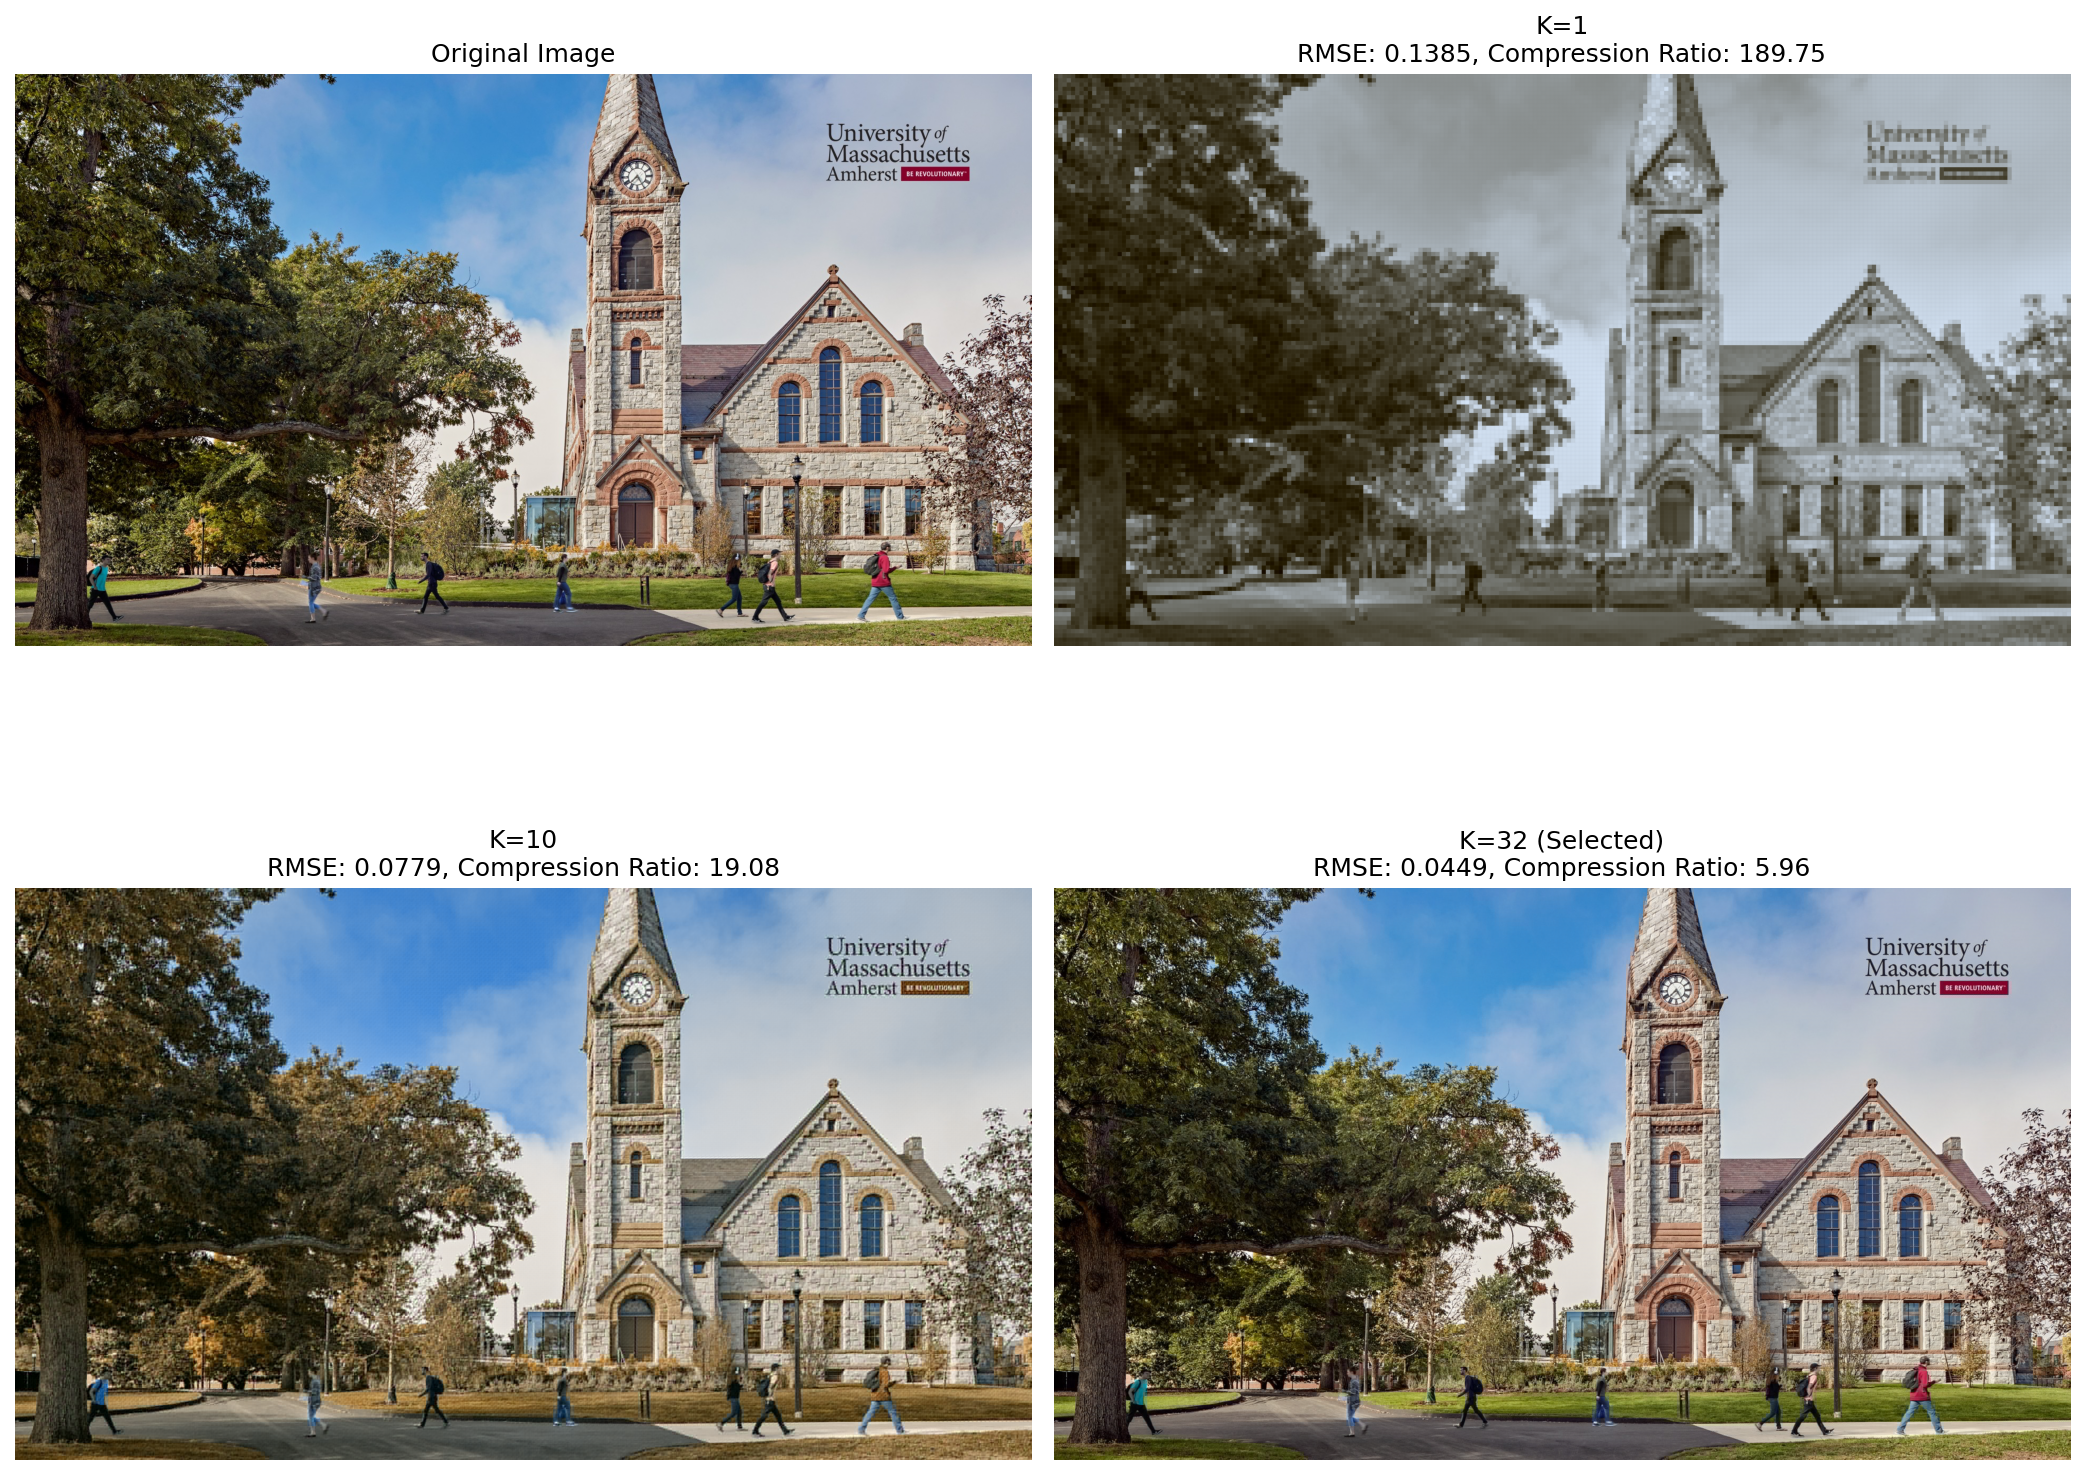
\includegraphics[width=0.95\textwidth]{reconstructions.png}
\caption{Comparison of reconstructed images: Original (top-left), $K=1$ (top-right), $K=10$ (bottom-left), and $K=32$ (bottom-right).}
\label{fig:q3e}
\end{figure}

\noindent
\textbf{Selected Value of $K$:} I selected $K = 32$ as the smallest value that produces a reconstruction perceptually indistinguishable from the original image.

\begin{table}[H]
\centering
\begin{tabular}{|c|c|c|}
\hline
\textbf{Metric} & \textbf{Value} \\
\hline
Selected $K$ & 32 \\
\hline
Reconstruction RMSE & 0.0449 \\
\hline
Compression Ratio & 5.96 \\
\hline
\end{tabular}
\caption{Summary of results for the selected value of $K$.}
\label{tab:q3e}
\end{table}

\noindent
My observation is that this choice of $K = 32$ represents a good balance between compression (nearly 6:1 ratio) and visual quality. Using 32 principal components retains approximately $32/192 \approx 16.7\%$ of the original patch dimensionality while preserving the perceptual quality of the image.

\section*{Question 4: Generative AI Disclosure}

I used generative AI tools to assist with debugging and understanding Python syntax for the coding portions of Questions 1, 2, and 3. Specifically, I used it to help with NumPy array operations and matplotlib plotting functions. 

\end{document}